% In the batch queue,  queue time becomes dominant but, at the same time, we
% have more freedom to decide the parameters of the slot.

\subsection{Experiments}\label{sec:ngeExp}

We designed experiments to characterize the performance of the NGE on Titan,
with an emphasis on understanding its overhead and thus the cost of introducing
new functionalities.  We perform three groups of experiments in which we
investigate the weak scalability, weak scalability with multiple generation, and
strong scalability of the NGE.

Each experiment entails executing multiple instances of AthenaMP using the NGE
to simulate a pre-determined number of events. All the experiments have been
performed by  configuring AthenaMP to use all the 16 cores  of Titan's worker
nodes.

We  measured the execution time of the pilots and of the AthenaMP  executed
within them, collecting timestamps at  all stages of the execution. Experiments
have been performed  by  submitting NGE's pilots  to Titan's batch queue.  The
turnaround time of an individual run is determined by queue waiting times. Since
we are interested only in the performances of the NGE, we removed queue time
from our statistics.

\subsubsection{Weak scalability}

In this experiment  we run as many AthenaMP instances (hereafter referred to as
tasks)  as the number of nodes controlled by the pilot. Each AthenaMP simulates
100 events, requiring $\sim 4200$ seconds on average.

Tasks do not  wait within the NGE Agent's queue since  one node  is available to
each AthenaMP instance.  Overheads in task execution are consequence primarily
of the three other factors: (i) the  initial bootstrapping of the pilot on the
nodes; (ii) the UnitManager's dispatching of  units (tasks) to the agent; and
(iii) time for the agent to bootstrap all the tasks on the nodes.

We tested  pilots  with 250, 500, 1000 and 2000 worker nodes and 2 hours
walltime. The time duration is determined by the Titan's walltime policy.
Figure~\ref{fig:weakScal1a} depicts the average pilot duration, the average
execution time of AthenaMP, and the NGE pilot overhead as function of the pilot
size.

\begin{figure}[!htb]
        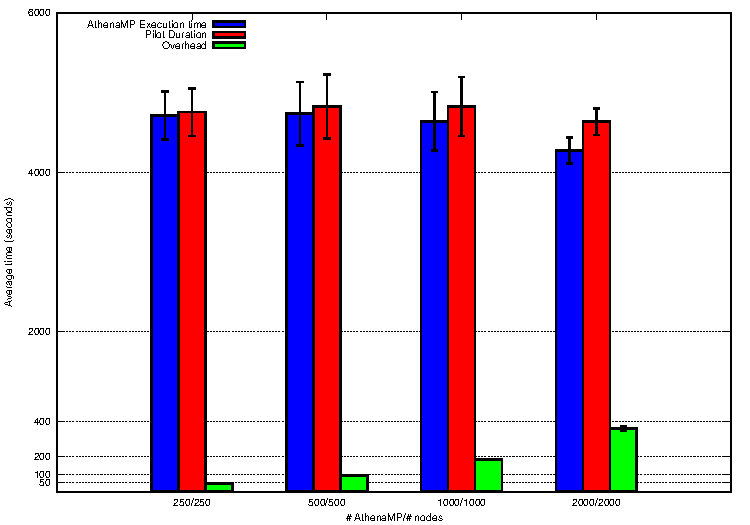
\includegraphics[height=4.5cm,width=\columnwidth]{./figures/NGE/weak1.pdf}
    \caption{Weak scalability: average pilot duration, average  duration of a
    single AthenaMP execution, and pilot's overhead as a function of different pilot sizes (200, 500, 1000 and 2000 nodes).}
\label{fig:weakScal1a}
\end{figure}

We observe that, despite some fluctuations due to external factors (e.g.,
Titan's shared filesystem and the shared database used by the NGE), the average
execution time of AthenaMP  ranges between 4200 and 4800 seconds.  We  also
observe that in all the cases the gap between AthenaMP execution times and the
pilot durations is minimal, although it slightly increases with the pilot size.
We  notice that NGE's overhead does grow linearly with the number of units.

%\begin{figure}[!htb]
%        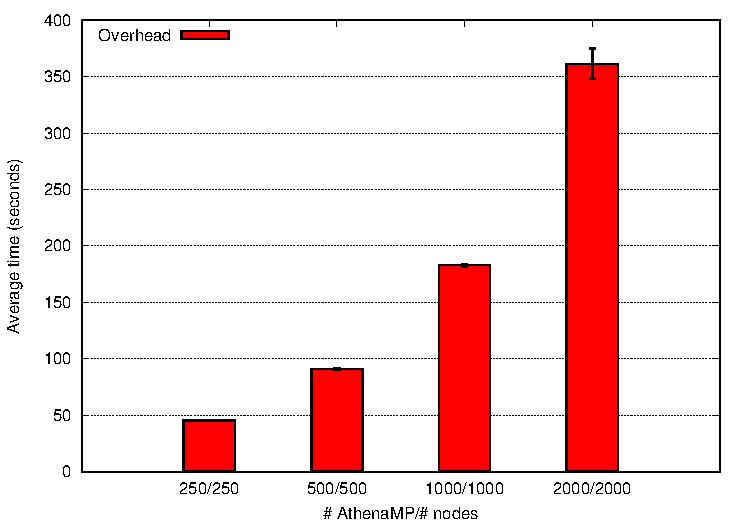
\includegraphics[width=0.4\textwidth]{./figures/NGE/weakOver1.pdf}
%    \caption{Weak scalability: average overhead by running AthenaMP on 200, 500, 1000 and 2000 nodes.}
%\label{fig:weakScal1b}
%\end{figure}

\subsubsection{Weak scalability with multiple generation }

The NGE provides an important new capability of submitting multiple generations
of AthenaMP to the same pilot. In order to investigate the cost of doing so, we
performed a variant of the weak scalability experiments. This stresses the
pilot's components, as new tasks are scheduled for execution on the Agent while
other tasks are still running.

% \mtnote{we dowe need to keep it below 2 hours?}\aanote{You are right. It was misleading. I Changed. Check if you like it.}

In these experiments, we run five AthenaMP instances per node.  As these
experiments are designed to investigate the overhead generated by the scheduling
and bootstrap of AthenaMP instances, we reduced the number of events simulated
by each AthenaMP task to sixteen in such a way that the running time of each
AthenaMP is, on average, $\sim 1200$ seconds. This experiment design choice does
not affect the  objectives or accuracy of the experiments, but allows us to
scale experiments to large node counts by being conservative with allocation.

% \footnote{Note that the number of events has been chosen in such a way
% that all the cores of a node run one event.}
%In this way, every core of each worker node was used to simulate one event,
%. This allows us to complete
%reducing the running time of each AthenaMP to ~$20$ minutes. % only.

We ran pilots with 256, 512, 1024 and 2048 worker nodes and 3\mtnote{2?} hours
walltime. Figure~\ref{fig:weakScal2a} depicts the average pilot duration, the
average execution time of five sequential generations of AthenaMP, and the
corresponding overhead. We observe that the difference between the two durations
is more marked than in the previous experiments. Despite this, we notice that
the growth of the overhead is consistent with the increment of the number of
tasks per node for pilots with 256, 512 and 1024 worker nodes, and less than
linear for the pilot with 2048 worker nodes.

\begin{figure}[!htb]
        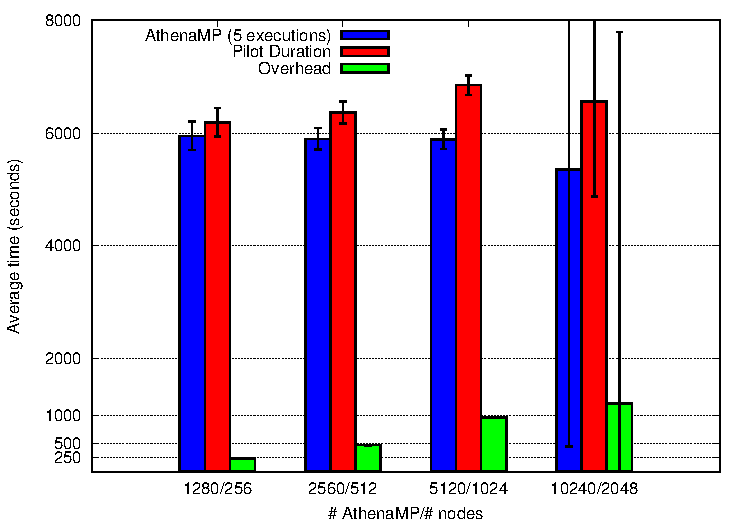
\includegraphics[height=4.5cm,width=\columnwidth]{./figures/NGE/weak2.pdf}
    \caption{Weak scalability with multiple generations: average pilot
    duration, average duration of five sequential AthenaMP executions, and
    pilot's overhead for different pilot sizes (256, 512, 1024 and 2048 nodes).}
\label{fig:weakScal2a}
\end{figure}

%\begin{figure}[!htb]
%        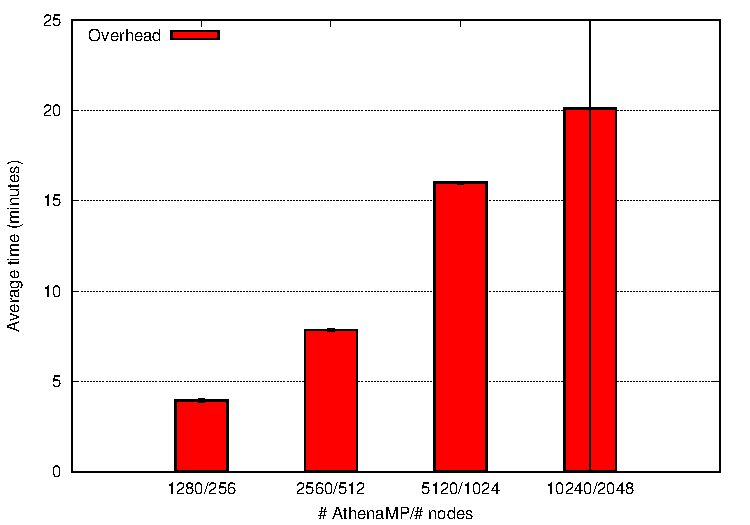
\includegraphics[width=0.4\textwidth]{./figures/NGE/weakOver2.pdf}
%    \caption{Weak scalability with multiple generations: average overhead by running AthenaMP on 256, 512, 1024 and 2048 nodes.}
%\label{fig:weakScal2b}
%\end{figure}


\subsubsection{Strong scalability}

The last experiments  study strong scalability by running the same number of
tasks for different pilot sizes. We used 2048 AthenaMP instances and  pilots
with 256, 512, 1024 and 2048 nodes. Thus, the number of AthenaMP generations is
equal to eight times the size of the smallest pilot and corresponds to the size
of the largest pilot. As a consequence, the number of consecutive generations of
AthenaMP decreases with the pilot size by generating different dynamics within
the pilots. These experiments are designed to investigate whether pilot overhead
is affected by the degree of concurrency within the pilot and/or the number of
tasks. Each AthenaMP instance simulates sixteen events as in the previous
experiment.

% \mtnote{Not sure I understand this sentence}\aanote{My fault. It should
% have been seven and null or 8 and 1. It depends on how we consider the word
% sequential. anyway, to avoid confusion I changed the sentence.}.

Figure \ref{fig:strongScala}  shows the average pilot duration and the average
execution time of possibly sequential AthenaMP instances.  We  notice that the
difference between the pilot duration and the AthenaMP execution times is almost
constant for all the pilot sizes, although the overall duration of the pilot
decreases linearly with the pilot size.

\begin{figure}[!htb]
        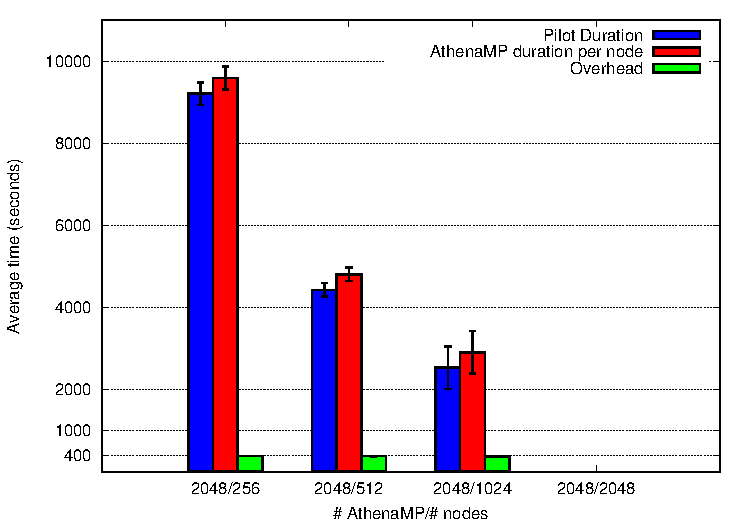
\includegraphics[height=4.5cm,width=\columnwidth]{./figures/NGE/strong.pdf}
    \caption{Strong scalability:  average pilot duration, average duration of
    sequential AthenaMP executions, and pilot's overhead for different pilot
    sizes (256, 512, 1024 and 2048 nodes).}
\label{fig:strongScala}
\end{figure}

%
%\begin{figure}[!htb]
%        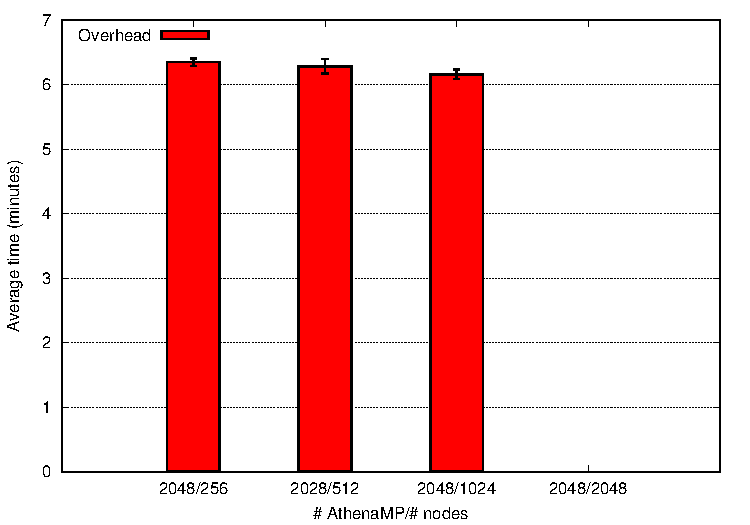
\includegraphics[width=0.4\textwidth]{./figures/NGE/strongOver.pdf}
%    \caption{Strong scalability: average overhead running AthenaMP on 256, 512, 1024 and 2048 nodes.}
%\label{fig:strongScalb}
%\end{figure}

%\subsubsection{Heterogeneous execution}
%
%The last experiment provides a proof of concept about the ability of the NGE to execute heterogeneous workload.
%In particular, we coupled the execution of AthenaMP with the execution of Gromacs to simulate molecular dynamics.
%We performed the experiment by executing at first one AthenaMP per node and then, submitting a Gromacs simulation per core. Each Gromacs simulation requires ~20 minutes.
%We tested the following pilot sizes : 8, 16, 32, 64.
%
%\begin{figure}[!htb]
%        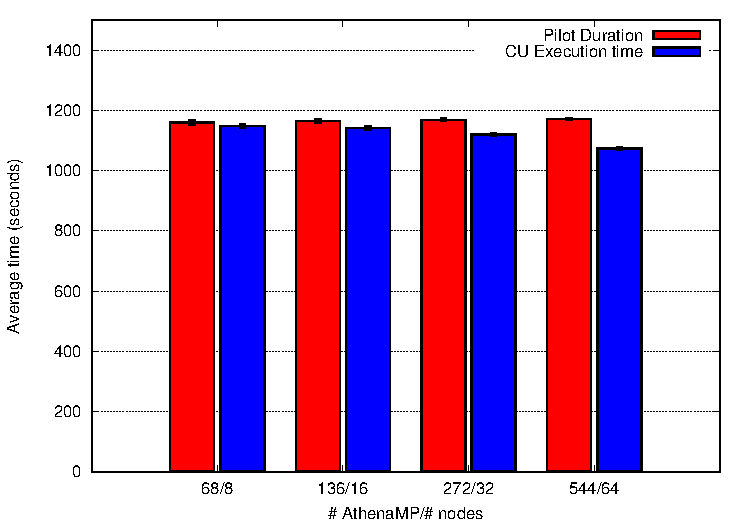
\includegraphics[width=0.5\textwidth]{./figures/NGE/MDET.pdf}
%    \caption{Average pilot execution time against average AthenaMP execution times  for pilot sizes: 256, 512, 1024 and 2048.}
%\label{fig:strongScala}
%\end{figure}
%\begin{figure}[!htb]
%        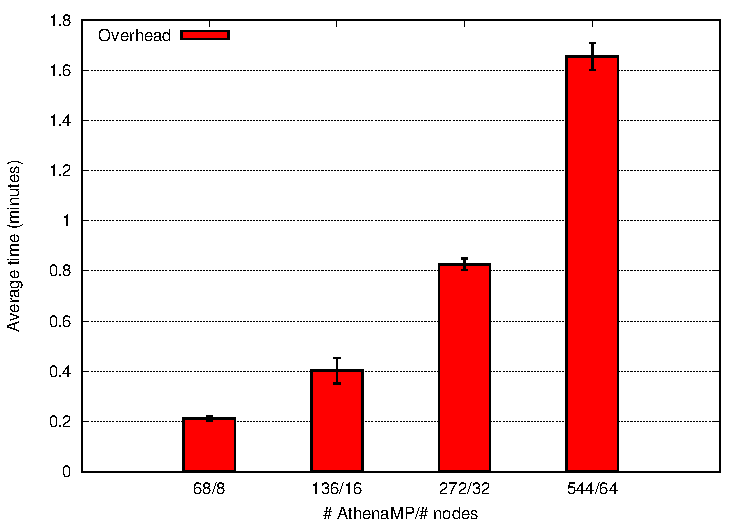
\includegraphics[width=0.5\textwidth]{./figures/NGE/MDOver.pdf}
%    \caption{Average overhead running AthenaMP for pilot sizes: 256, 512, 1024 and 2048.}
%\label{fig:MDScal}
%\end{figure}

% For this reason, the second set of the experiments aims to find
%sub-optimal parameters with which we can minimize the trade-off between the size
%of a slot and the time spent in queue waiting for that slot to become available.
%In other words, we aim to minimize the completion time by finding the best
%trade-off between execution time and queue time.
%
%This execution model introduces slot utilization as one of the key factors for
%high-performances. This happens because, in order to minimize the time spent in
%queue, we might asks for slots in advance and, then we could not be able to
%saturate them when they become available. Thus, this strategy requires a new
%functionality that allows the job to receive and execute new events while it is
%already running on the resources. In order to do that we perform the experiments
%by using a new generation executor that implements such functionality.
%
%As last observation, it is important to point out that the percentage of
%utilization of a slot is minor problem with the current implementation because,
%due to the dynamics of the Backfill queue, PanDA has a high probability to
%re-acquire a slot immediately after it has released one\aanote{Are we able to
%quantify this ``immediately''?}.
